\documentclass[11pt]{article}

% Self-contained: compiles on arXiv with a standard TeX Live, no external style files.
\usepackage[margin=1in]{geometry}
\usepackage[T1]{fontenc}
\usepackage{lmodern}
\usepackage{amsmath,amssymb}
\usepackage{graphicx}
\usepackage{booktabs}
\usepackage{siunitx}
\usepackage{xcolor}
\usepackage[colorlinks=true,allcolors=blue!60!black]{hyperref}
\usepackage{caption}
\captionsetup{font=small,labelfont=bf}

\graphicspath{{figs/}}

\title{\textbf{POISE: Hardware-State-Conditioned Variable-Depth\\
Inference on the Edge --- A Characterization}}

% TODO: fill in author name / affiliation before submission.
\author{[Author Name]\\ \texttt{imthiyas916@gmail.com}}
\date{\today}

\begin{document}
\maketitle

\begin{abstract}
We set out to build POISE, an on-device inference orchestrator that varies per-token
transformer depth in response to \emph{live hardware physics}---junction temperature, power,
and throttle status---so as to hold throughput and cut energy under sustained thermal load,
where a fixed-depth model throttles and collapses. We built the full apparatus: a
variable-depth engine, an on-board first-order RC thermal calibration, a PID controller that
maps thermal error to a layer budget, and an evaluation harness, and we measured the mechanism
end to end on an NVIDIA Jetson AGX Orin running an 8B-parameter decoder. \textbf{Our central
finding refutes the thermal premise for this platform.} Across single-stream decode,
long-context prefill, and batched inference, doubling the layer count moves steady-state power
by at most \SI{2}{\watt} (16$\to$32 layers) while throughput scales roughly $2\times$: on this
class of accelerator, depth is an \emph{energy/throughput knob, not a thermal actuator}. A PID
controller conditioned on junction temperature correctly sheds depth as the chip warms, yet
runs the \emph{hottest} of all configurations---because the shallower, faster model keeps the
GPU more continuously active, and depth does not modulate power. We report what
hardware-state-conditioned depth control \emph{does} deliver---${\sim}2\times$ throughput and
${\sim}2\times$ lower energy per token---at a measured, non-trivial quality cost, and we
characterize precisely why the thermal-regulation mechanism fails on a
memory-/power-ceiling-bound device. All numbers are eval-harness outputs on real hardware,
reported with variance; results that contradict the initial hypothesis are reported as found.
\end{abstract}

\section{Introduction}
Edge LLM inference is widely assumed to be thermally constrained: run a fixed-depth model on a
thermally-limited device under sustained load, and the junction heats up, the hardware throttles
the clock to protect the silicon, and throughput collapses. The POISE hypothesis was that an
engine could \emph{shed transformer layers when the device gets hot}---executing a variable
number of layers per token, a \emph{layer budget}, chosen from the device's measured physical
state---and thereby stay ahead of the throttle cliff.

We built the complete apparatus to test this and measured it end to end. This paper reports the
measurements, \emph{including the ones that contradict the hypothesis}. Our contribution is a
characterization: (i) a clean physical account of why depth fails as a thermal-control actuator
for decode on a power-ceiling-bound accelerator, and (ii) a quantification of what
hardware-state depth control does buy---throughput and energy---and at what quality cost.

We do not claim adaptive depth itself as novel. Existing early-exit / adaptive-depth
methods~\cite{calm,layerskip} condition execution depth on \emph{input difficulty} (token or
sequence confidence, content). The angle we studied is the \emph{hardware-state} loop; the axes
are orthogonal and composable.

\section{Related work}
Input-difficulty adaptive computation is a mature line: CALM~\cite{calm} exits early per token
from confidence estimates; LayerSkip~\cite{layerskip} trains a model with layer dropout and an
early-exit loss so shallow exits stay usable; a broader early-exit literature conditions depth on
content and entropy. These decide depth from \emph{what is being computed}. POISE instead
conditions depth on \emph{the state of the hardware doing the computing} (temperature, power,
clock, throttle). The two are composable; here we isolate and measure the hardware-state loop.
We use a LoRA adapter~\cite{lora} for the early-exit adaptation step, evaluate on
ARC~\cite{arc}, and run an 8B DeepSeek-R1-Distill-Llama model~\cite{deepseekr1}.

\section{Method}
\paragraph{Variable-depth execution.} For each generated token, the engine runs the forward pass
through decoder layers $0\ldots b{-}1$ for a chosen budget $b$, then projects the depth-$b$
hidden state to logits via the model's final norm and LM head. Constant-budget generation is
bit-identical to standard decoding; the runner contains no control logic (mechanism vs.\ policy
separation).

\paragraph{On-board thermal calibration.} A load driver sustains fixed-depth inference while
sampling telemetry, producing one heating trace per depth. We fit a first-order RC model,
\begin{equation}
\frac{dT}{dt} = \frac{1}{C_{\text{th}}}\!\left(P - \frac{T - T_{\text{amb}}}{R_{\text{th}}}\right),
\end{equation}
from the warm-up curves. The fit is accurate: $R_{\text{th}}=\SI{0.807}{\kelvin\per\watt}$,
$C_{\text{th}}=\SI{87.6}{\joule\per\kelvin}$, $\tau=\SI{64.8}{\second}$, RMSE
$\SI{0.32}{\celsius}$. The thermal \emph{model} is accurate; as we show, the \emph{mechanism} is
what fails.

\paragraph{Control.} A PID controller maps thermal error (setpoint minus measured junction
temperature) to a layer budget, with an unconditional thermal-safety override. An anticipatory
PPO tier was designed but not pursued (Section~\ref{sec:discussion}).

\section{Experimental setup}
Model: DeepSeek-R1-Distill-Llama-8B (32 layers, \texttt{fp16}, eager attention). Device: NVIDIA
Jetson AGX Orin, MAXN power mode, \texttt{jtop} telemetry. Quality: per-depth multiple-choice
accuracy on 300 AI2 ARC items (150 easy + 150 challenge) via length-normalized log-likelihood
scoring (standard \texttt{acc\_norm}); we also report KL divergence, perplexity, and top-1
agreement versus the full-32 model. Throughput / energy: sustained generation with real
telemetry, energy per token $=\int P\,dt / \text{tokens}$, steady-state tails,
$\geq 3$ repeats. Compute-bound regimes are measured by slicing the decoder to $b$ layers and
running sustained prefill (sequence 2048) and batched (\(8\times512\)) forwards.

\section{Results}

\subsection{Depth is an energy/throughput knob}
Halving the layer count roughly doubles throughput and halves energy per token
(Figure~\ref{fig:tradeoff}a, Table~\ref{tab:bench}), with negligible run-to-run variance
(std $<\SI{0.1}{tok/s}$). Since $\text{tok/s}\cdot\text{W}^{-1} = 1/(\text{J}\cdot\text{tok}^{-1})$,
depth-16 delivers $2.05\times$ the throughput-per-watt of depth-32.

\begin{table}[h]
\centering
\small
\begin{tabular}{rrrrr}
\toprule
depth & tok/s & J/token & tok/s$\cdot$W$^{-1}$ & ARC acc \\
\midrule
32 (full) & 12.09 & 3.90 & 0.257 ($1.00\times$) & 0.557 \\
28 & 13.80 & 3.41 & 0.293 ($1.14\times$) & 0.477 \\
24 & 15.97 & 2.92 & 0.342 ($1.33\times$) & 0.423 \\
16 & 23.95 & 1.90 & \textbf{0.527} ($\mathbf{2.05\times}$) & 0.347 \\
\bottomrule
\end{tabular}
\caption{Per-depth throughput, energy, and quality on the Jetson (MAXN, $\geq3$ repeats).
Energy/throughput scale ${\sim}2\times$; ARC accuracy (LayerSkip adapter) falls steeply.}
\label{tab:bench}
\end{table}

\subsection{The quality cost is real}
Depth reduction is not free (Figure~\ref{fig:tradeoff}b). On ARC, shedding to depth-28 costs
14\% relative accuracy, depth-24 costs 24\%, and depth-16 costs 38\%---all far above the
$\leq$2--3\% the project initially hoped for. A LoRA early-exit adapter lifts the whole curve by
2--5 points and does not damage full-depth accuracy, but opens no ``free'' reduced-depth band.
(The distributional KL signal \emph{overstated} the collapse: it flags depth-28 as unusable,
yet that depth's task-accuracy loss is only ${\sim}14\%$.)

\begin{figure}[t]
\centering
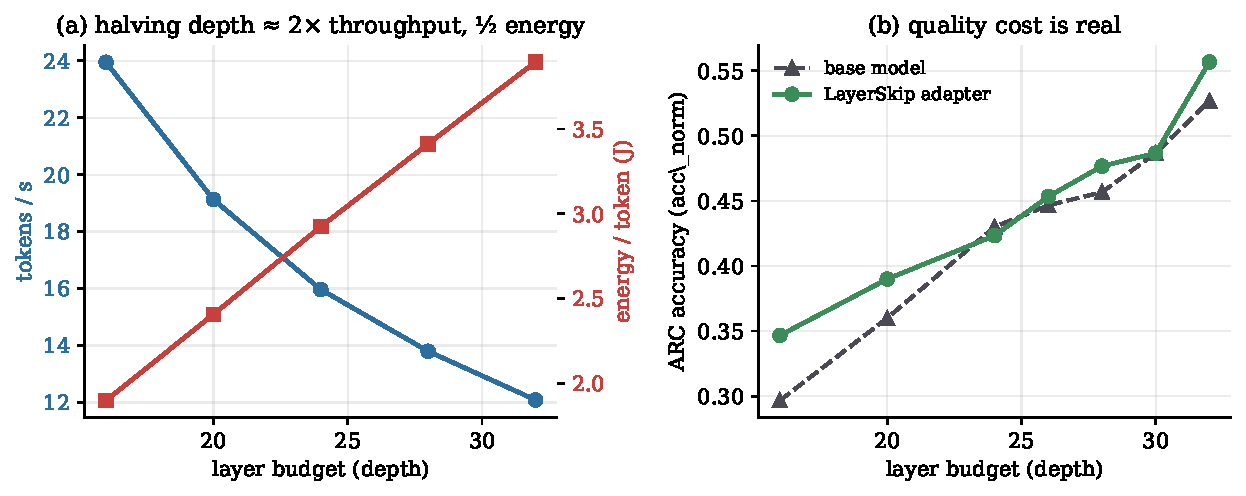
\includegraphics[width=\textwidth]{fig_tradeoff.pdf}
\caption{\textbf{The trade-off.} (a) Halving depth $\approx 2\times$ throughput and
$\tfrac12$ energy per token. (b) The quality cost is real; the LayerSkip adapter shifts the
curve up modestly but opens no free band.}
\label{fig:tradeoff}
\end{figure}

\subsection{Power is flat across depth---in every regime}
The decisive physical result: doubling depth barely moves power (Figure~\ref{fig:flatpower}). In
single-stream decode, $\Delta P \approx \SI{2}{\watt}$ over 16$\to$32 layers; in long-context
prefill, $\SI{1.2}{\watt}$; in batched forwards, $\SI{0.9}{\watt}$. Throughput meanwhile scales
${\sim}2\times$. At MAXN the module runs at a power/clock ceiling for any heavy workload, so
additional layers take proportionally longer at the \emph{same} power. Depth does not modulate
heat, in any regime we tested.

\begin{figure}[t]
\centering
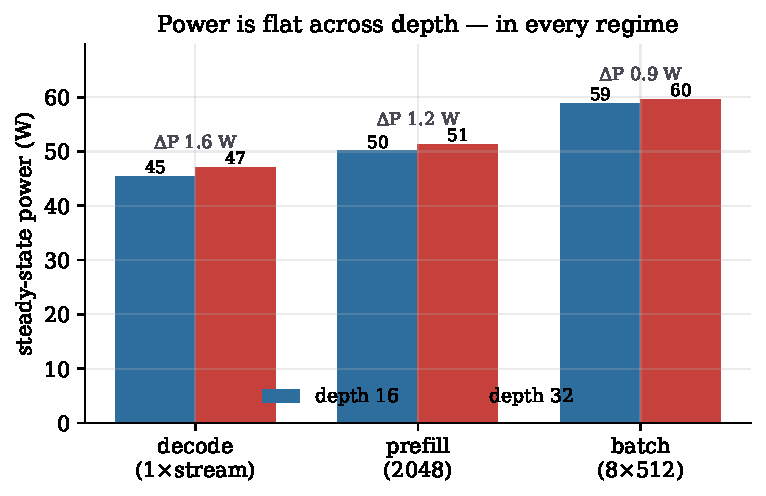
\includegraphics[width=0.62\textwidth]{fig_flatpower.pdf}
\caption{\textbf{Flat power.} Steady-state power at depth 16 vs.\ 32 across decode, prefill, and
batched forwards. The gap is $\leq\SI{2}{\watt}$ everywhere, while throughput scales ${\sim}2\times$.}
\label{fig:flatpower}
\end{figure}

\subsection{On-board closed loop: depth is not a thermal actuator}
We ran static-32, static-16, and PID (setpoint \SI{50}{\celsius}) under sustained load for
\SI{130}{\second} each (Table~\ref{tab:stress}, Figure~\ref{fig:thermal}). Three facts settle
the hypothesis: (i) \textbf{static-16 runs hotter than static-32} despite half the depth, because
$2\times$ throughput keeps the GPU more continuously active; (ii) \textbf{PID correctly sheds
depth} ($32\to21$) once junction temperature exceeds setpoint, yet runs the \emph{hottest} of
the three---the actuator has no authority over the variable it targets; (iii) at
${\sim}\SI{47}{\watt}$ the chip plateaus near \SI{60}{\celsius} and never approaches the
${\sim}\SI{87}{\celsius}$ passive-throttle point, so there is no throttle to avoid.

\begin{table}[h]
\centering
\small
\begin{tabular}{lrrrr}
\toprule
mode & tok/s & peak $T_j$ (\si{\celsius}) & mean depth & J/token \\
\midrule
static-32 & 11.74 & 60.8 & 32.0 & 4.07 \\
static-16 & 23.23 & \textbf{62.2} & 16.0 & 2.04 \\
PID       & 18.74 & \textbf{62.7} & 20.9 & 2.55 \\
\bottomrule
\end{tabular}
\caption{Closed-loop stress test (setpoint \SI{50}{\celsius}, \SI{130}{\second}/mode). The
shallower and adaptive configurations run \emph{hotter}, not cooler.}
\label{tab:stress}
\end{table}

\begin{figure}[t]
\centering
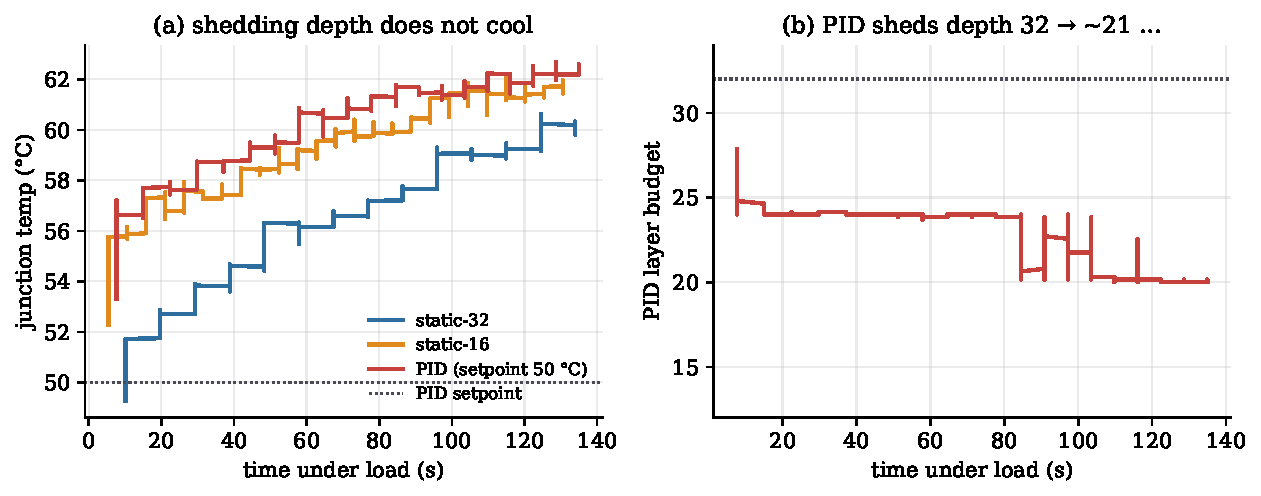
\includegraphics[width=\textwidth]{fig_thermal.pdf}
\caption{\textbf{Shedding depth does not cool.} (a) Junction temperature over time: full-depth
static-32 is the \emph{coolest}; static-16 and PID run hotter. (b) The PID controller actively
sheds its budget from 32 toward ${\sim}21$---and still runs hottest.}
\label{fig:thermal}
\end{figure}

\section{Discussion}
\label{sec:discussion}
On the Jetson Orin, hardware-state-conditioned depth control is an \emph{energy-per-token /
throughput knob}, not a thermal governor. The realizable value: at a fixed operating point,
reducing depth yields ${\sim}$linear throughput and energy gains at a measured, non-trivial
quality cost, so a controller can pick the depth that meets a latency or energy target for the
current workload. It cannot regulate temperature, because on this class of accelerator power is
bound by a memory/clock/power ceiling that depth does not move---a property of the
hardware$\times$workload, not of the controller, and one that holds identically across decode,
prefill, and batched inference. Consequently we did not pursue PPO: trained against a simulator
whose depth$\to$power map is flat, the policy has no thermal signal to learn. Whether any
accelerator/workload regime exists where depth moves power enough to regulate temperature
remains open; it is not this platform in any regime we tested.

\section{Limitations}
The thermal-regulation objective as originally framed is \emph{not supported} by our
measurements; we report it as refuted rather than narrowing the claim silently. ARC scored by
MC-likelihood underrates a chain-of-thought model in absolute terms, so we rely on the per-depth
\emph{deltas}, which are internally consistent. We measure a single device (one AGX Orin) in
MAXN mode; a hard \texttt{nvpmodel} power cap requires a reboot and, given flat depth$\to$power,
would not create a differential thermal benefit. Any ``neuromorphic-inspired'' analogy, if used,
refers only to hardware-state-conditioned variable-depth execution---never a silicon claim.

\section{Conclusion}
We asked whether shedding transformer layers can keep an edge LLM ahead of thermal throttling,
built the full system to test it, and measured a clean answer: on a Jetson Orin, depth is an
energy/throughput knob, not a thermal one. The negative result is decisive and reproducible, and
the positive finding---${\sim}2\times$ throughput and energy per token from hardware-state depth
control, at a quantified quality cost---is what the mechanism honestly offers.

\paragraph{Reproducibility.} Calibration, quality gate, throughput/energy benchmark,
closed-loop stress test, and the compute-bound probe are scripted; all figures regenerate from
committed result files via \texttt{docs/arxiv/make\_figures.py}.

\begin{thebibliography}{9}
\bibitem{calm} T.~Schuster, A.~Fisch, J.~Gupta, et al. Confident Adaptive Language Modeling.
\emph{NeurIPS}, 2022.
\bibitem{layerskip} M.~Elhoushi, A.~Shrivastava, D.~Liskovich, et al. LayerSkip: Enabling Early
Exit Inference and Self-Speculative Decoding. \emph{ACL}, 2024.
\bibitem{lora} E.~J.~Hu, Y.~Shen, P.~Wallis, et al. LoRA: Low-Rank Adaptation of Large Language
Models. \emph{ICLR}, 2022.
\bibitem{arc} P.~Clark, I.~Cowhey, O.~Etzioni, et al. Think you have Solved Question Answering?
Try ARC, the AI2 Reasoning Challenge. \emph{arXiv:1803.05457}, 2018.
\bibitem{deepseekr1} DeepSeek-AI. DeepSeek-R1: Incentivizing Reasoning Capability in LLMs via
Reinforcement Learning. \emph{arXiv:2501.12948}, 2025.
\end{thebibliography}

\end{document}
